% !TEX program = lualatex
% Source: ../../2025/week6/week6.pdf (18 slides) and week6.ipynb.
\documentclass[12pt,aspectratio=43]{beamer}
% Shared Beamer design. Load after \documentclass using \input.
% Engine: LuaLaTeX. Fonts: UD Digi Kyokasho N (regular/bold), Arial.
\usepackage{luatexja-fontspec}
\setmainjfont[BoldFont={UD Digi Kyokasho N Bold}]{UD Digi Kyokasho N}
\setsansjfont[BoldFont={UD Digi Kyokasho N Bold}]{UD Digi Kyokasho N}
\setmonojfont[BoldFont={UD Digi Kyokasho N Bold}]{UD Digi Kyokasho N}
% Liberation Sans keeps the layout usable on systems without Arial.
\IfFontExistsTF{Arial}{
  \setmainfont{Arial}
  \setsansfont{Arial}
  \setmonofont{Arial}
}{
  \setmainfont{Liberation Sans}
  \setsansfont{Liberation Sans}
  \setmonofont{Liberation Sans}
}
\renewcommand{\kanjifamilydefault}{\gtdefault}

% Typeset mathematics with a dedicated TeX math font, independent of Arial.
\usefonttheme{professionalfonts}
\usepackage[mathrm=sym]{unicode-math}
\setmathfont{Latin Modern Math}
\setoperatorfont{\symup}

\definecolor{courseblue}{HTML}{4472C4}
\definecolor{ruleblue}{HTML}{8FAADC}
\setbeamercolor{normal text}{fg=black,bg=white}
\setbeamercolor{structure}{fg=courseblue}
\setbeamercolor{frametitle}{fg=black,bg=white}
\setbeamercolor{title banner}{fg=white,bg=courseblue}
\setbeamerfont{frametitle}{size=\fontsize{18}{22}\selectfont,series=\mdseries}
\setbeamerfont{quote}{shape=\upshape}
\setbeamersize{text margin left=9mm,text margin right=9mm}
\setbeamertemplate{navigation symbols}{}
\setbeamercolor{page number}{fg=gray,bg=white}
\setbeamertemplate{footline}{%
  \begin{beamercolorbox}[wd=\paperwidth,ht=2.5mm,dp=1.5mm]{page number}
    \hfill{\fontsize{8}{9}\selectfont
      \ifnum\value{framenumber}>0
        \insertframenumber\,/\,\inserttotalframenumber
      \fi}\hspace*{3mm}
  \end{beamercolorbox}}
\setbeamertemplate{headline}{%
  \hfill\textcolor{gray}{\fontsize{6}{7}\selectfont
    \hypersetup{linkcolor=gray}% Keep Beamer's title links in the header color.
    \ifnum\value{framenumber}=0 \insertshortdate\enspace\fi
    \insertshorttitle\space\insertshortsubtitle}\hspace{2mm}\vspace{1.5mm}}
\setbeamertemplate{frametitle}{%
  \vspace{2mm}\centering\insertframetitle\par
  \vspace{-1mm}{\color{ruleblue}\rule{.44\paperwidth}{.5pt}}\par
  \vspace{2mm}}
\setbeamercolor{itemize item}{fg=courseblue}
\setbeamercolor{itemize subitem}{fg=black}
\setbeamercolor{itemize subsubitem}{fg=black}
\setbeamertemplate{itemize item}{\textbullet}
\setbeamertemplate{itemize subitem}{\textnormal{-}}
\setbeamertemplate{itemize subsubitem}{\textnormal{-}}
\setlength{\parskip}{.45em}
\hypersetup{colorlinks=true,urlcolor=courseblue}

% Use \titlepage inside a [t,noframenumbering] frame. The background extends
% 1 mm past both page edges to avoid hairline gaps in PDF viewers.
\setbeamertemplate{title page}{%
  \vspace{2mm}
  \begin{beamercolorbox}[wd=\paperwidth,ht=43mm,dp=13mm,colsep*=1mm,center]{title banner}
    {\fontsize{32}{40}\selectfont\inserttitle\par}
    \vspace{2mm}
    {\fontsize{20}{24}\selectfont\insertsubtitle\par}
  \end{beamercolorbox}
  \vspace{10mm}
  \hfill\insertauthor
}

\graphicspath{{figures/}}
\usepackage{listings}
\usepackage{upquote}
\IfFontExistsTF{Consolas}{\newfontfamily\codefont{Consolas}}{\newfontfamily\codefont{Liberation Mono}}
\definecolor{codevalue}{HTML}{7A3E9D}
\definecolor{codebuiltin}{HTML}{006DB0}
\definecolor{codestring}{HTML}{267348}
\newcommand{\code}[1]{{\codefont #1}}
\lstdefinestyle{python}{
  language=Python,
  basicstyle=\codefont\fontsize{12}{14}\selectfont,
  keywordstyle=\color{codebuiltin},
  keywordstyle=[2]\color{codebuiltin},
  morekeywords=[2]{print,range},
  stringstyle=\color{codestring},
  showstringspaces=false,
  columns=fullflexible,
  keepspaces=true,
  upquote=true,
  tabsize=4,
  breaklines=false,
  backgroundcolor=\color{black!4},
  frame=single,framerule=0pt,framesep=1.7mm,
  xleftmargin=1.7mm,xrightmargin=1.7mm,
  aboveskip=1mm,belowskip=0.5mm,
  literate=*{0}{{{\color{codevalue}0}}}1
    {1}{{{\color{codevalue}1}}}1 {2}{{{\color{codevalue}2}}}1
    {3}{{{\color{codevalue}3}}}1 {4}{{{\color{codevalue}4}}}1
    {5}{{{\color{codevalue}5}}}1 {6}{{{\color{codevalue}6}}}1
    {7}{{{\color{codevalue}7}}}1 {8}{{{\color{codevalue}8}}}1
    {9}{{{\color{codevalue}9}}}1
}
\lstset{style=python}
\setbeamercolor{lesson note}{fg=black,bg=courseblue!9}
\newenvironment{lessonbox}
  {\begin{beamercolorbox}[wd=\linewidth,sep=1.5mm]{lesson note}}
  {\end{beamercolorbox}\par}

\title{計算物理学B}
\subtitle{第六回：数値微分}
\author{野垣 康介、藤本 悠輝}
\date{2026/11/24}
\hypersetup{pdftitle={計算物理学B 第六回：数値微分},pdfauthor={野垣 康介、藤本 悠輝}}

\begin{document}

\begin{frame}[t,noframenumbering]
  \titlepage
\end{frame}

\begin{frame}{講義予定}
  \setlength{\parskip}{0pt}
  2026年度 第2学期（火曜3限）
  \par\vspace{2mm}
  \begingroup\centering
    \renewcommand{\arraystretch}{1.05}
    \begin{tabular}{@{}l@{\hspace{2mm}}l@{\hspace{4mm}}l@{\hspace{2mm}}l@{}}
      10/6 & 四則演算 & 12/8 & モンテカルロ1 \\
      10/27 & 制御文（for, if） & 12/15 & モンテカルロ2 \\
      11/6（金） & 関数 & 12/22 & 微分方程式1 \\
      11/10 & 配列（NumPy） & 1/12 & 微分方程式2 \\
      11/17 & 可視化（matplotlib） & 1/19 & 偏微分方程式1 \\
      \textcolor{courseblue}{\textbf{11/24}} & \textcolor{courseblue}{\textbf{数値微分}} & 1/26 & 偏微分方程式2 \\
      12/1 & 数値積分 & 2/2 & 根の探索 \\
      \multicolumn{2}{c}{\small ～中間レポート～} & \multicolumn{2}{c}{\small ～期末レポート～}
    \end{tabular}\par
  \endgroup
  \vspace{2mm}
  {\small 10/20は出張で休講。11/6（金）は火曜授業の振替。\par}
  \vspace{1mm}
  {\fontsize{7}{8}\selectfont 日付：\href{https://www.niigata-u.ac.jp/wp-content/uploads/2025/08/schedule_2026.pdf}{令和8年度（2026）新潟大学授業暦}\par}
\end{frame}

\begin{frame}[t]{講義資料とノートブック}
  \begin{itemize}
    \setlength{\itemsep}{3mm}
    \item Google Colab：{\small\url{https://colab.research.google.com/?hl=ja}}
    \item 講義資料：{\small\url{https://github.com/nogaki/Computational_Physics_B}}
    \item 今週の教材：\code{2026/week6/}
    \item 編集できるスライド：\code{slide.tex}
    \item 実習ノートブック：\code{week6.ipynb}
  \end{itemize}
  \vspace{2mm}
  GitHubからノートブックを開いたら、Colabの「ファイル」メニューから\textbf{ドライブにコピーを保存}します。
\end{frame}

\begin{frame}[t]{今日の内容}
  \begin{itemize}
    \setlength{\itemsep}{3mm}
    \item 浮動小数点数と丸め誤差
    \item 前進差分・後退差分・中心差分
    \item 刻み幅 $h$ と打ち切り誤差・桁落ち
    \item 関数の変化の速さによる誤差の違い
  \end{itemize}
  \vfill
  \begin{lessonbox}
    数値微分では、公式の次数を上げるだけでなく、\textbf{刻み幅を適切に選ぶ}ことが必要です。
  \end{lessonbox}
\end{frame}

\begin{frame}[t]{計算機上の数}
  \begin{itemize}
    \setlength{\itemsep}{2mm}
    \item 計算機は、有限個の0と1（bit）で数を表します。
    \item Pythonの\code{float}は、通常64 bitの倍精度浮動小数点数です。
    \item Pythonの整数型は任意精度で、浮動小数点数とは表し方が異なります。
  \end{itemize}
  \vspace{2mm}
  2進数では、各桁が $2$ のべきの重みを持ちます。
  \[
    (1101)_2=1\cdot2^3+1\cdot2^2+0\cdot2^1+1\cdot2^0=13
  \]
  \small 8 bitでは1 byteです。整数の格納方法には符号付き表現などがあります。
\end{frame}

\begin{frame}[t]{負の整数：2の補数}
  \setlength{\parskip}{1mm}
  8 bitの2の補数表現では、最上位bitの重みが負になります。
  \[
    (b_7b_6\cdots b_0)_2=-b_7 2^7+\sum_{k=0}^{6} b_k2^k
  \]
  \begin{columns}[c,onlytextwidth]
    \begin{column}{.47\textwidth}
      \centering
      \code{00000101}$_2=5$
    \end{column}
    \begin{column}{.47\textwidth}
      \centering
      \code{11111011}$_2=-5$
    \end{column}
  \end{columns}
  \vspace{3mm}
  \begin{lessonbox}
    $M$ bitの2の補数で表せる範囲は $-2^{M-1}$ から $2^{M-1}-1$ です。
  \end{lessonbox}
\end{frame}

\begin{frame}[t]{浮動小数点数}
  \begin{itemize}
    \setlength{\itemsep}{2mm}
    \item IEEE 754 binary64は符号1 bit・指数部11 bit・格納仮数部52 bitです。
    \item 正規化数では暗黙の先頭1 bitを含め、有効桁は53 bitです。
    \item 多くの実数は有限桁に丸めて保存します。
  \end{itemize}
  \[
    \pm (0.b_1b_2\cdots b_p)_2\times 2^e
  \]
  たとえば10進数の $0.1$ は2進数で循環します。
  \[
    0.1=(0.0001100110011\ldots)_2
  \]
\end{frame}

\begin{frame}[t,fragile]{0.1の表現を確認する}
  \setlength{\parskip}{0pt}
  \code{float}では有限桁に丸められた値が保存されています。
\begin{lstlisting}
a = 0.1
print(f"{a:.55f}")
\end{lstlisting}
  \vspace{2mm}
  表示例：
  \[
    0.10000000000000000555\ldots
  \]
  \begin{lessonbox}
    表示された余分な桁は、計算機が近似値を保持していることを示します。
  \end{lessonbox}
\end{frame}

\begin{frame}[t,fragile]{繰り返し加算と丸め誤差}
  同じ小数を繰り返し足しても、数学上の値と計算結果は完全には一致しないことがあります。
\begin{lstlisting}
total = 0.0
for _ in range(10_000_000):
    total += 0.01
print(total)
\end{lstlisting}
  \vspace{1mm}
  数値計算では、丸め誤差が反復回数とともに積み重なる場合があります。
  \begin{itemize}
    \item 精度が必要な総和には、補償和などの方法もあります。
    \item まずは結果の桁数や収束を確かめます。
  \end{itemize}
\end{frame}

\begin{frame}[t]{情報落ちと桁落ち}
  \begin{columns}[t,onlytextwidth]
    \begin{column}{.48\textwidth}
      \textbf{情報落ち：大きさが違う数の加算}
      \[
        10^{16}+1
      \]
      小さい数の情報が丸めで失われることがあります。
    \end{column}
    \begin{column}{.48\textwidth}
      \textbf{桁落ち：近い数の減算}
      \[
        1.0000001-1.0000000
      \]
      近い値の差では、相対的な誤差が大きくなりえます。
    \end{column}
  \end{columns}
  \vspace{3mm}
  \begin{lessonbox}
    数値微分では、分子の差が小さくなるため、桁落ちが刻み幅の選択に影響します。
  \end{lessonbox}
\end{frame}

\begin{frame}[t,fragile]{テイラー展開から差分公式へ}
  $f$が十分滑らかなとき、
  \[
    f(x+h)=f(x)+hf'(x)+\frac{h^2}{2}f''(x)+O(h^3).
  \]
  $h$を小さくして差をとると、導関数を近似できます。
\begin{lstlisting}
(f(x + h) - f(x)) / h
\end{lstlisting}
  \vspace{1mm}
  ただし、$h$を小さくしすぎると、丸め誤差が増えます。
\end{frame}

\begin{frame}[t]{前進差分・後退差分・中心差分}
  \setlength{\parskip}{1mm}
  \[
    D_+f(x)=\frac{f(x+h)-f(x)}{h}=f'(x)+O(h)
  \]
  \[
    D_-f(x)=\frac{f(x)-f(x-h)}{h}=f'(x)+O(h)
  \]
  \[
    D_0f(x)=\frac{f(x+h)-f(x-h)}{2h}=f'(x)+O(h^2)
  \]
  \begin{itemize}
    \item 前進・後退差分：評価点の片側だけを使う。
    \item 中心差分：両側を使い、滑らかな関数では打ち切り誤差が小さい。
  \end{itemize}
\end{frame}

\begin{frame}[t]{二階微分の中心差分}
  前進差分・中心差分と同じように、左右対称な3点から二階微分を近似できます。
  \[
    f''(x)=\frac{f(x+h)-2f(x)+f(x-h)}{h^2}+O(h^2)
  \]
  \begin{itemize}
    \item 分子は、一次の変化が相殺されるように組み合わせています。
    \item 十分滑らかな関数では、打ち切り誤差は$O(h^2)$です。
  \end{itemize}
\end{frame}

\begin{frame}[t]{刻み幅 $h$ と2種類の誤差}
  \begin{columns}[t,onlytextwidth]
    \begin{column}{.48\textwidth}
      \textbf{打ち切り誤差}
      \begin{itemize}
        \item 差分公式を有限個の項で近似する誤差。
        \item $h$を小さくすると減る。
      \end{itemize}
    \end{column}
    \begin{column}{.48\textwidth}
      \textbf{丸め誤差}
      \begin{itemize}
        \item 浮動小数点演算による誤差。
        \item 差を$h$で割るため、小さい$h$で増えやすい。
      \end{itemize}
    \end{column}
  \end{columns}
  \vspace{2mm}
  \begin{lessonbox}
    誤差全体は$h$に対して谷を作ります。小さすぎず、大きすぎない刻み幅を探します。
  \end{lessonbox}
\end{frame}

\begin{frame}[t]{$\sin x$の数値微分}
  $x=0.3\pi$での真の微分係数は $\cos(0.3\pi)$ です。
  \begin{center}
    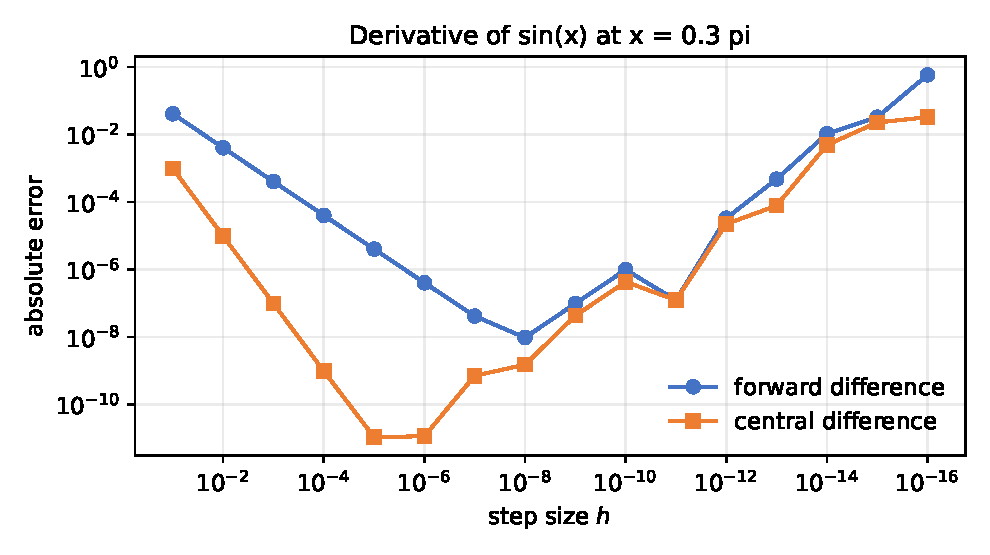
\includegraphics[width=.82\linewidth,height=41mm,keepaspectratio]{differentiation_error.pdf}
  \end{center}
  \small 前進差分は大きな$h$で打ち切り誤差が目立ち、小さな$h$では丸め誤差が目立ちます。
\end{frame}

\begin{frame}[t]{刻み幅の目安}
  倍精度浮動小数点数の機械精度は $\epsilon\approx 2.2\times10^{-16}$ です。
  \begin{itemize}
    \setlength{\itemsep}{3mm}
    \item 前進差分では、打ち切り誤差$O(h)$と丸め誤差$O(\epsilon/h)$が競合します。
    \item 中心差分では、打ち切り誤差$O(h^2)$と丸め誤差$O(\epsilon/h)$が競合します。
  \end{itemize}
  \[
    h_{\rm forward}\sim \epsilon^{1/2}\approx 10^{-8},\qquad
    h_{\rm central}\sim \epsilon^{1/3}\approx 10^{-5}
  \]
  \small これは関数や評価点に依存する目安で、普遍的な最適値ではありません。
\end{frame}

\begin{frame}[t,fragile]{刻み幅を変えて誤差を調べる}
  \setlength{\parskip}{0pt}
  \small 真値を知る関数で、$h$ごとの絶対誤差を比べます。
\begin{lstlisting}
x = 0.3 * np.pi
h = 10.0 ** (-np.arange(1, 17))
exact = np.cos(x)
forward = (np.sin(x + h) - np.sin(x)) / h
central = (
    np.sin(x + h) - np.sin(x - h)
) / (2 * h)
error_forward = np.abs(forward - exact)
error_central = np.abs(central - exact)
\end{lstlisting}
  \vspace{2mm}
  \small Notebookでは前進差分の誤差の谷を確認し、演習で中心差分と比べます。
\end{frame}

\begin{frame}[t]{関数が速く変化する場合}
  \setlength{\parskip}{1mm}
  $f(x)=\sin(\omega x)$では、導関数の大きさは$\omega$に比例し、高階導関数はさらに大きくなります。
  \[
    f'(x)=\omega\cos(\omega x),\qquad f'''(x)=-\omega^3\cos(\omega x)
  \]
  \begin{itemize}
    \item 打ち切り誤差の係数が変わるため、最適な$h$も変わります。
    \item $\omega=1$と$\omega=10^4$で、誤差を実際に比較します。
    \item 絶対誤差だけでなく、微分係数の大きさに対する相対誤差も確認します。
  \end{itemize}
\end{frame}

\begin{frame}[t,fragile]{実習：多項式の微分}
  \setlength{\parskip}{0pt}
  $f(x)=x^3-2x+1$の解析解は$f'(x)=3x^2-2$です。
\begin{lstlisting}
def f(x):
    return x**3 - 2*x + 1

def df_exact(x):
    return 3*x*x - 2
\end{lstlisting}
  \vspace{2mm}
  \begin{itemize}
    \item $x=0.7$で差分近似を計算し、解析解と比べます。
    \item $h$を変え、前進差分・中心差分の誤差を記録します。
  \end{itemize}
\end{frame}

\begin{frame}[t]{実習：振動関数と差分公式}
  \begin{enumerate}
    \setlength{\itemsep}{4mm}
    \item $\sin(10^4x)$を数値微分し、$\sin x$の場合と$h$の最適域を比べます。
    \item 前進差分・後退差分・中心差分を同じグラフに描きます。
    \item $h$を極端に小さくしたときの誤差を観察します。
  \end{enumerate}
  \vfill
  \begin{lessonbox}
    解析解を持つ関数で、近似値と誤差の両方を確かめましょう。
  \end{lessonbox}
\end{frame}

\begin{frame}[t]{まとめ}
  \begin{itemize}
    \setlength{\itemsep}{3mm}
    \item 浮動小数点数は有限精度で、丸め誤差が生じます。
    \item 近い数の減算では桁落ちが起こりやすくなります。
    \item 中心差分は滑らかな関数に対して$O(h^2)$の打ち切り誤差を持ちます。
    \item $h$を小さくしすぎると丸め誤差が増えるため、誤差を実際に調べます。
  \end{itemize}
  \vfill
  次回：数値積分
\end{frame}

\end{document}
